\subsection{Ultimate Guitar}
UltimateGuitar\cite{ultimateguitar_home} es una aplicación web diseñada específicamente para guitarra, aunque tambien ofrece soporte para otros instrumentos como el ukelele, el bajo y el piano. Aunque podemos encontrar páginas dedicadas a artículos, libros y un foro, destacamos las relacionadas con canciones y los cursos.

En primer lugar, con respecto a las \textbf{páginas relacionadas con canciones}, podemos encontrar:
\begin{itemize}
    \item \textbf{Biblioteca de canciones} (véase Figura~\ref{fig:ultimateguitar_home}), con la posibilidad de realizar búsquedas avanzadas por género, artista, popularidad y tipo (acordes, tablatura, instrumento\dots).
    \item \textbf{Canciones} (véase Figura~\ref{fig:ultimateguitar_somewhereovertherainbow}) que contienen la letra, acordes y utilidades~(véase Tabla~\ref{tab:ultimateguitar_utilidades_canciones}) para la práctica de las mismas.
\end{itemize}


En segundo lugar, en cuanto a los \textbf{cursos} (véase Figura~\ref{fig:ultimateguitar_courses}), Ultimate Guitar ofrece un catálogo de cursos para usuarios de distintos niveles. Estos incluyen vídeos, ejercicios interactivos y material descargable.

\begin{figure}[H]
    \centering
    % Primera fila
    \begin{subfigure}[t]{0.48\textwidth}
         \centering
        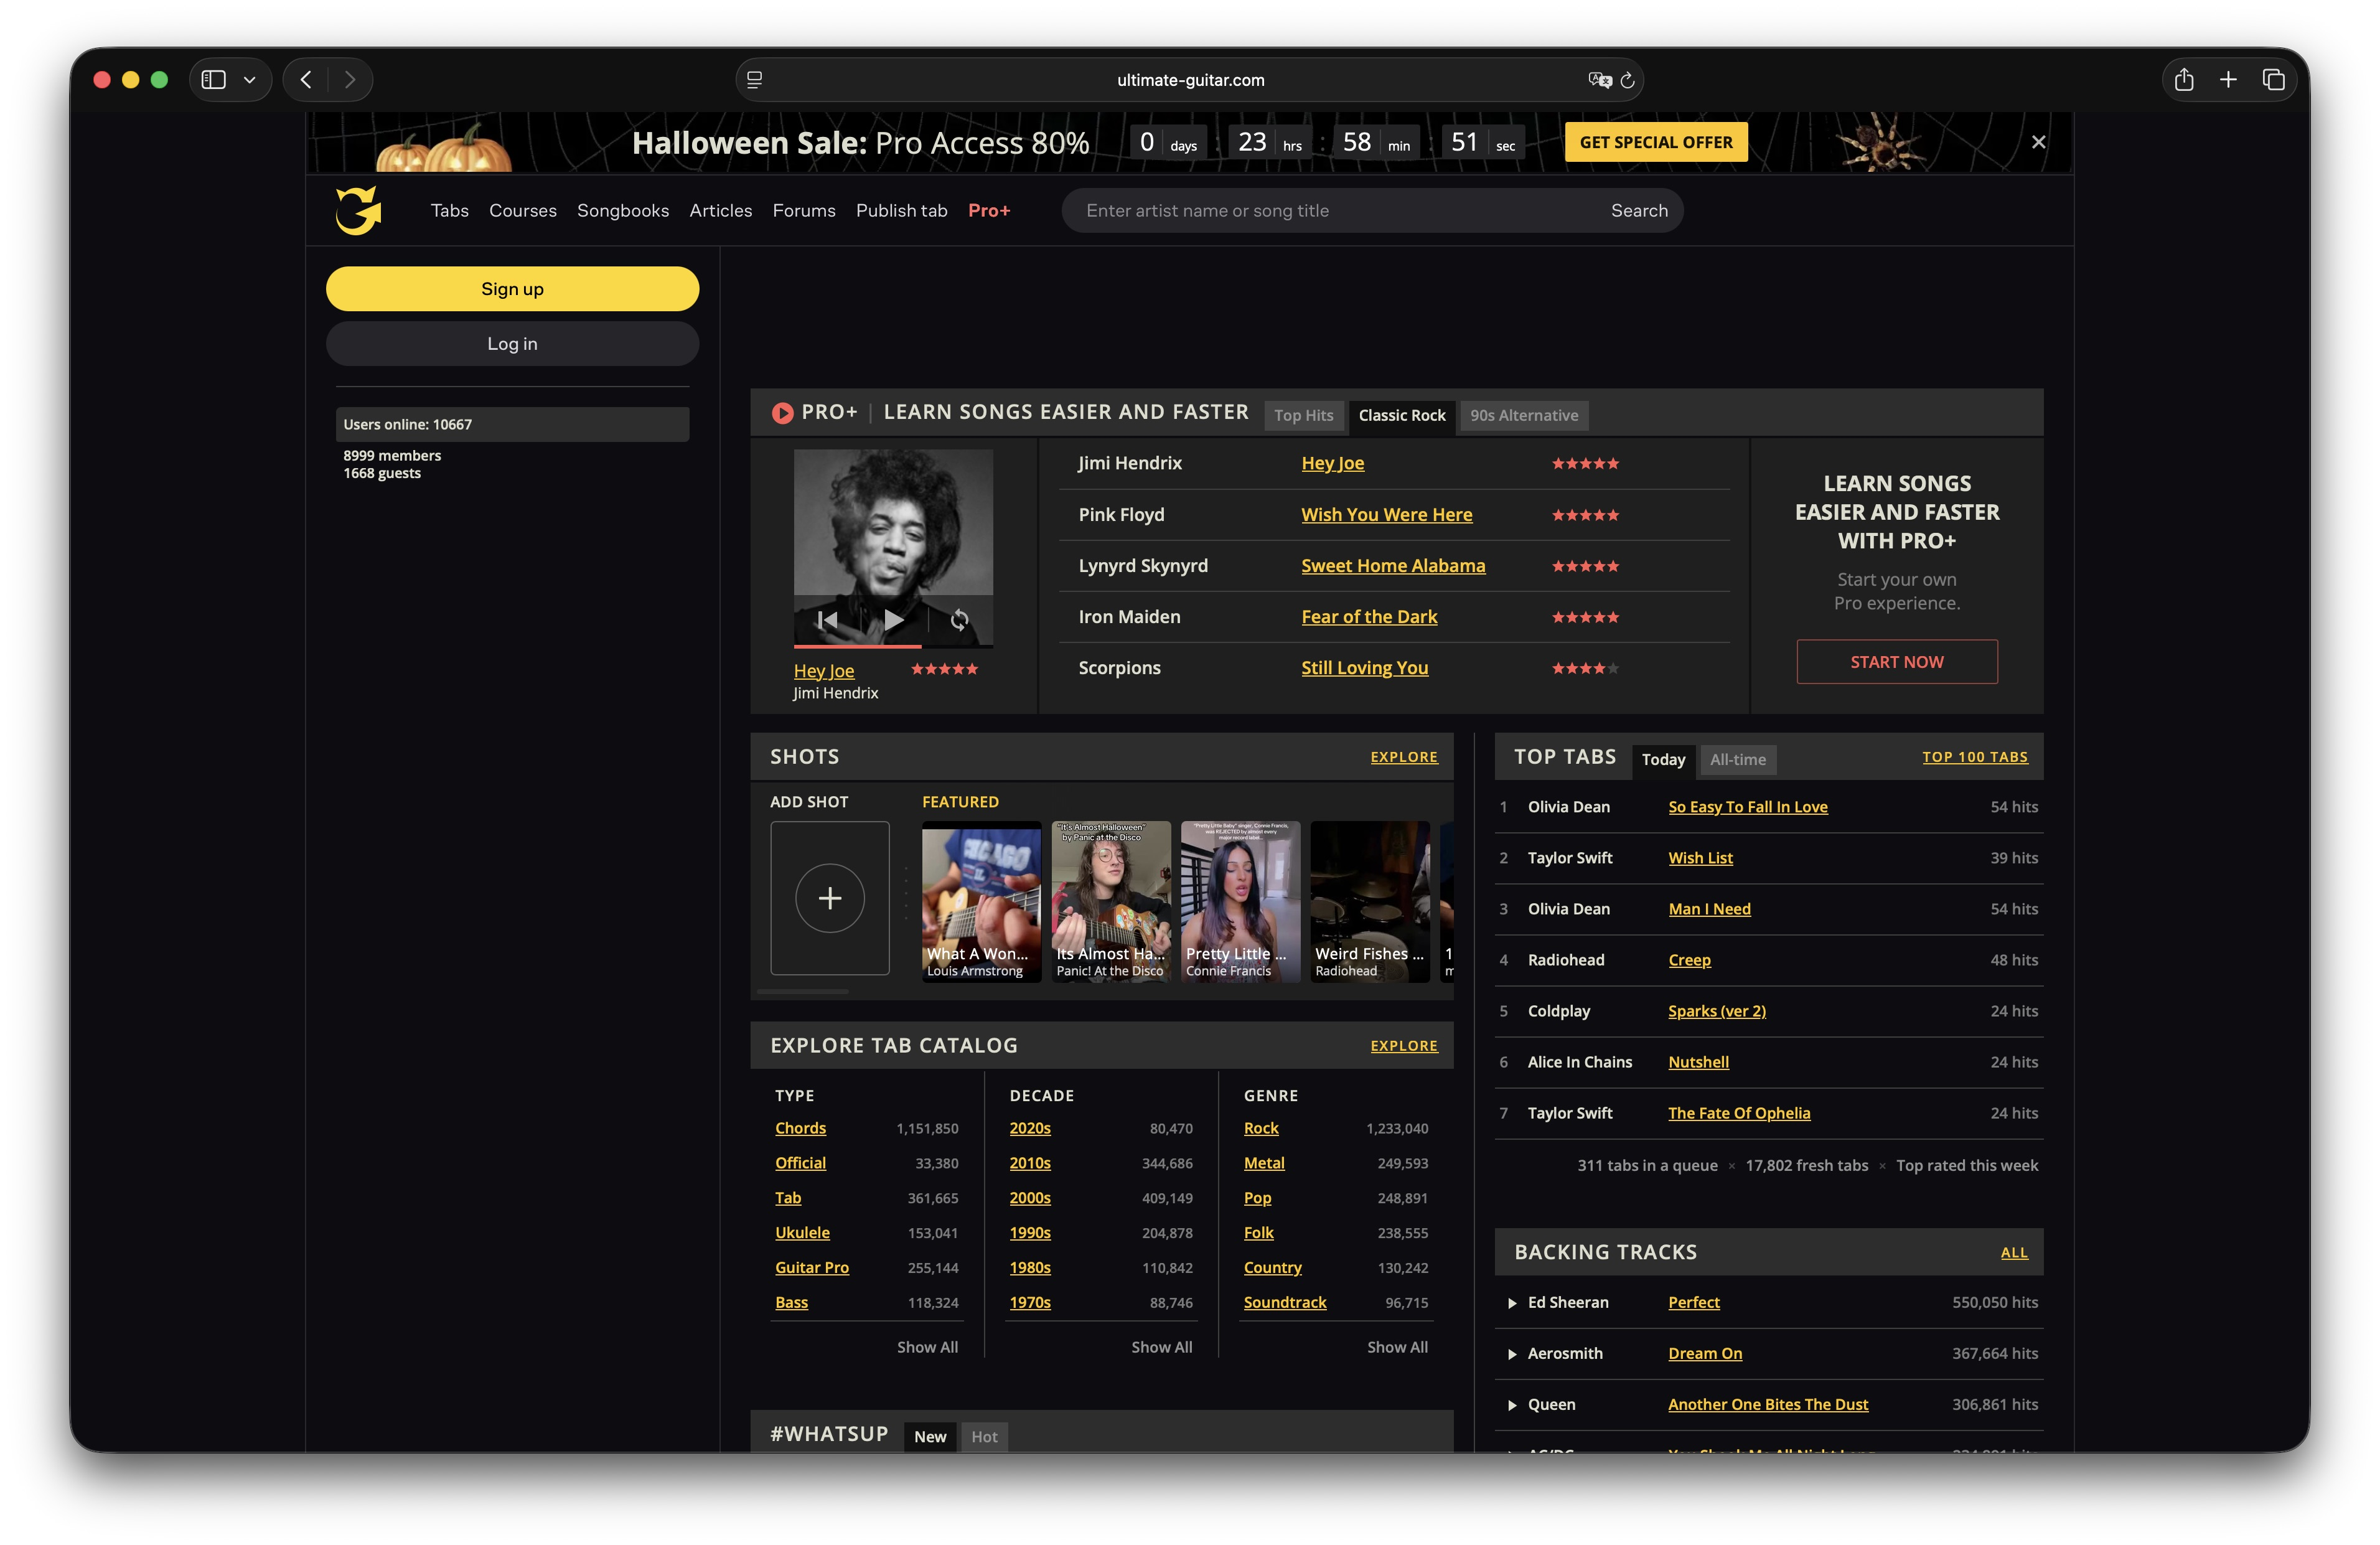
\includegraphics[width=\textwidth]{Ilustraciones/estado/ultimateguitar.jpeg}
        \caption{Página principal de Ultimate Guitar~\cite{ultimateguitar_home}}\label{fig:ultimateguitar_home}
    \end{subfigure}
    \hfill
    \begin{subfigure}[t]{0.48\textwidth}
        \centering
        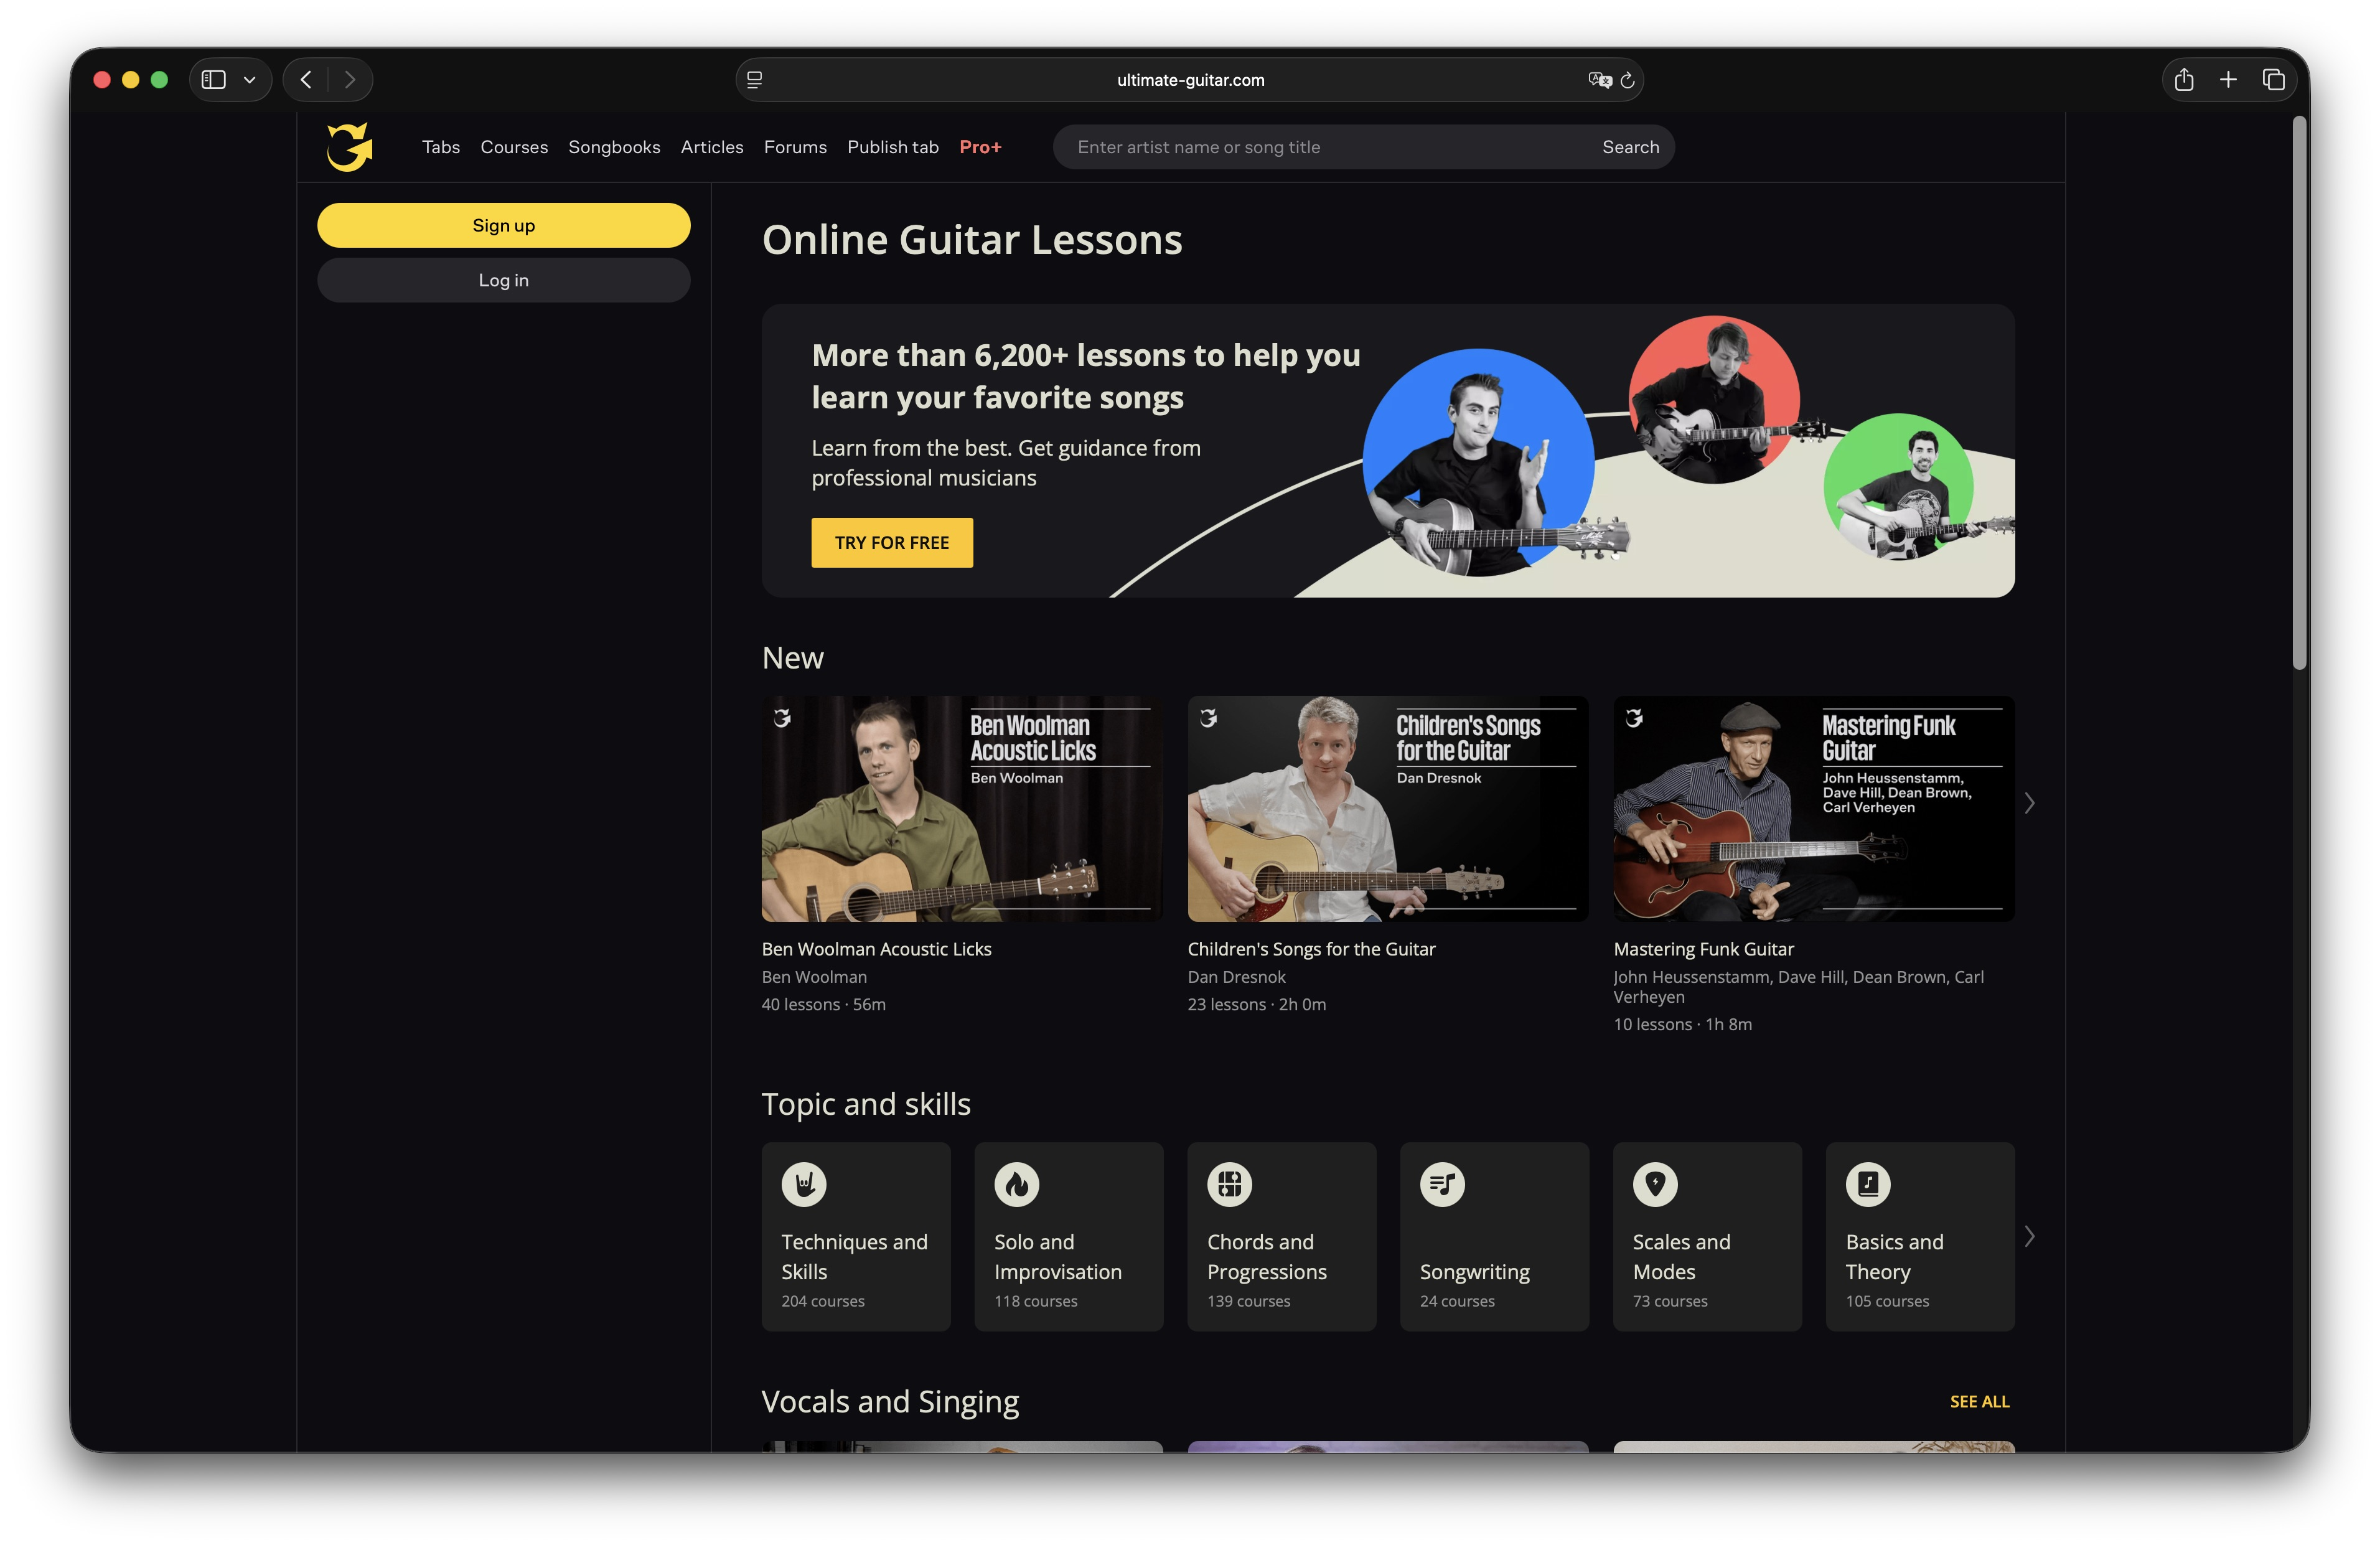
\includegraphics[width=\textwidth]{Ilustraciones/estado/ultimateguitar_courses.jpeg}
        \caption{Página de cursos de Ultimate Guitar~\cite{ultimateguitar_courses}}
        \label{fig:ultimateguitar_courses}
    \end{subfigure}
    \vspace{1em} % Espacio vertical entre filas

    % Segunda fila
    \begin{subfigure}[t]{\textwidth}
        \centering
        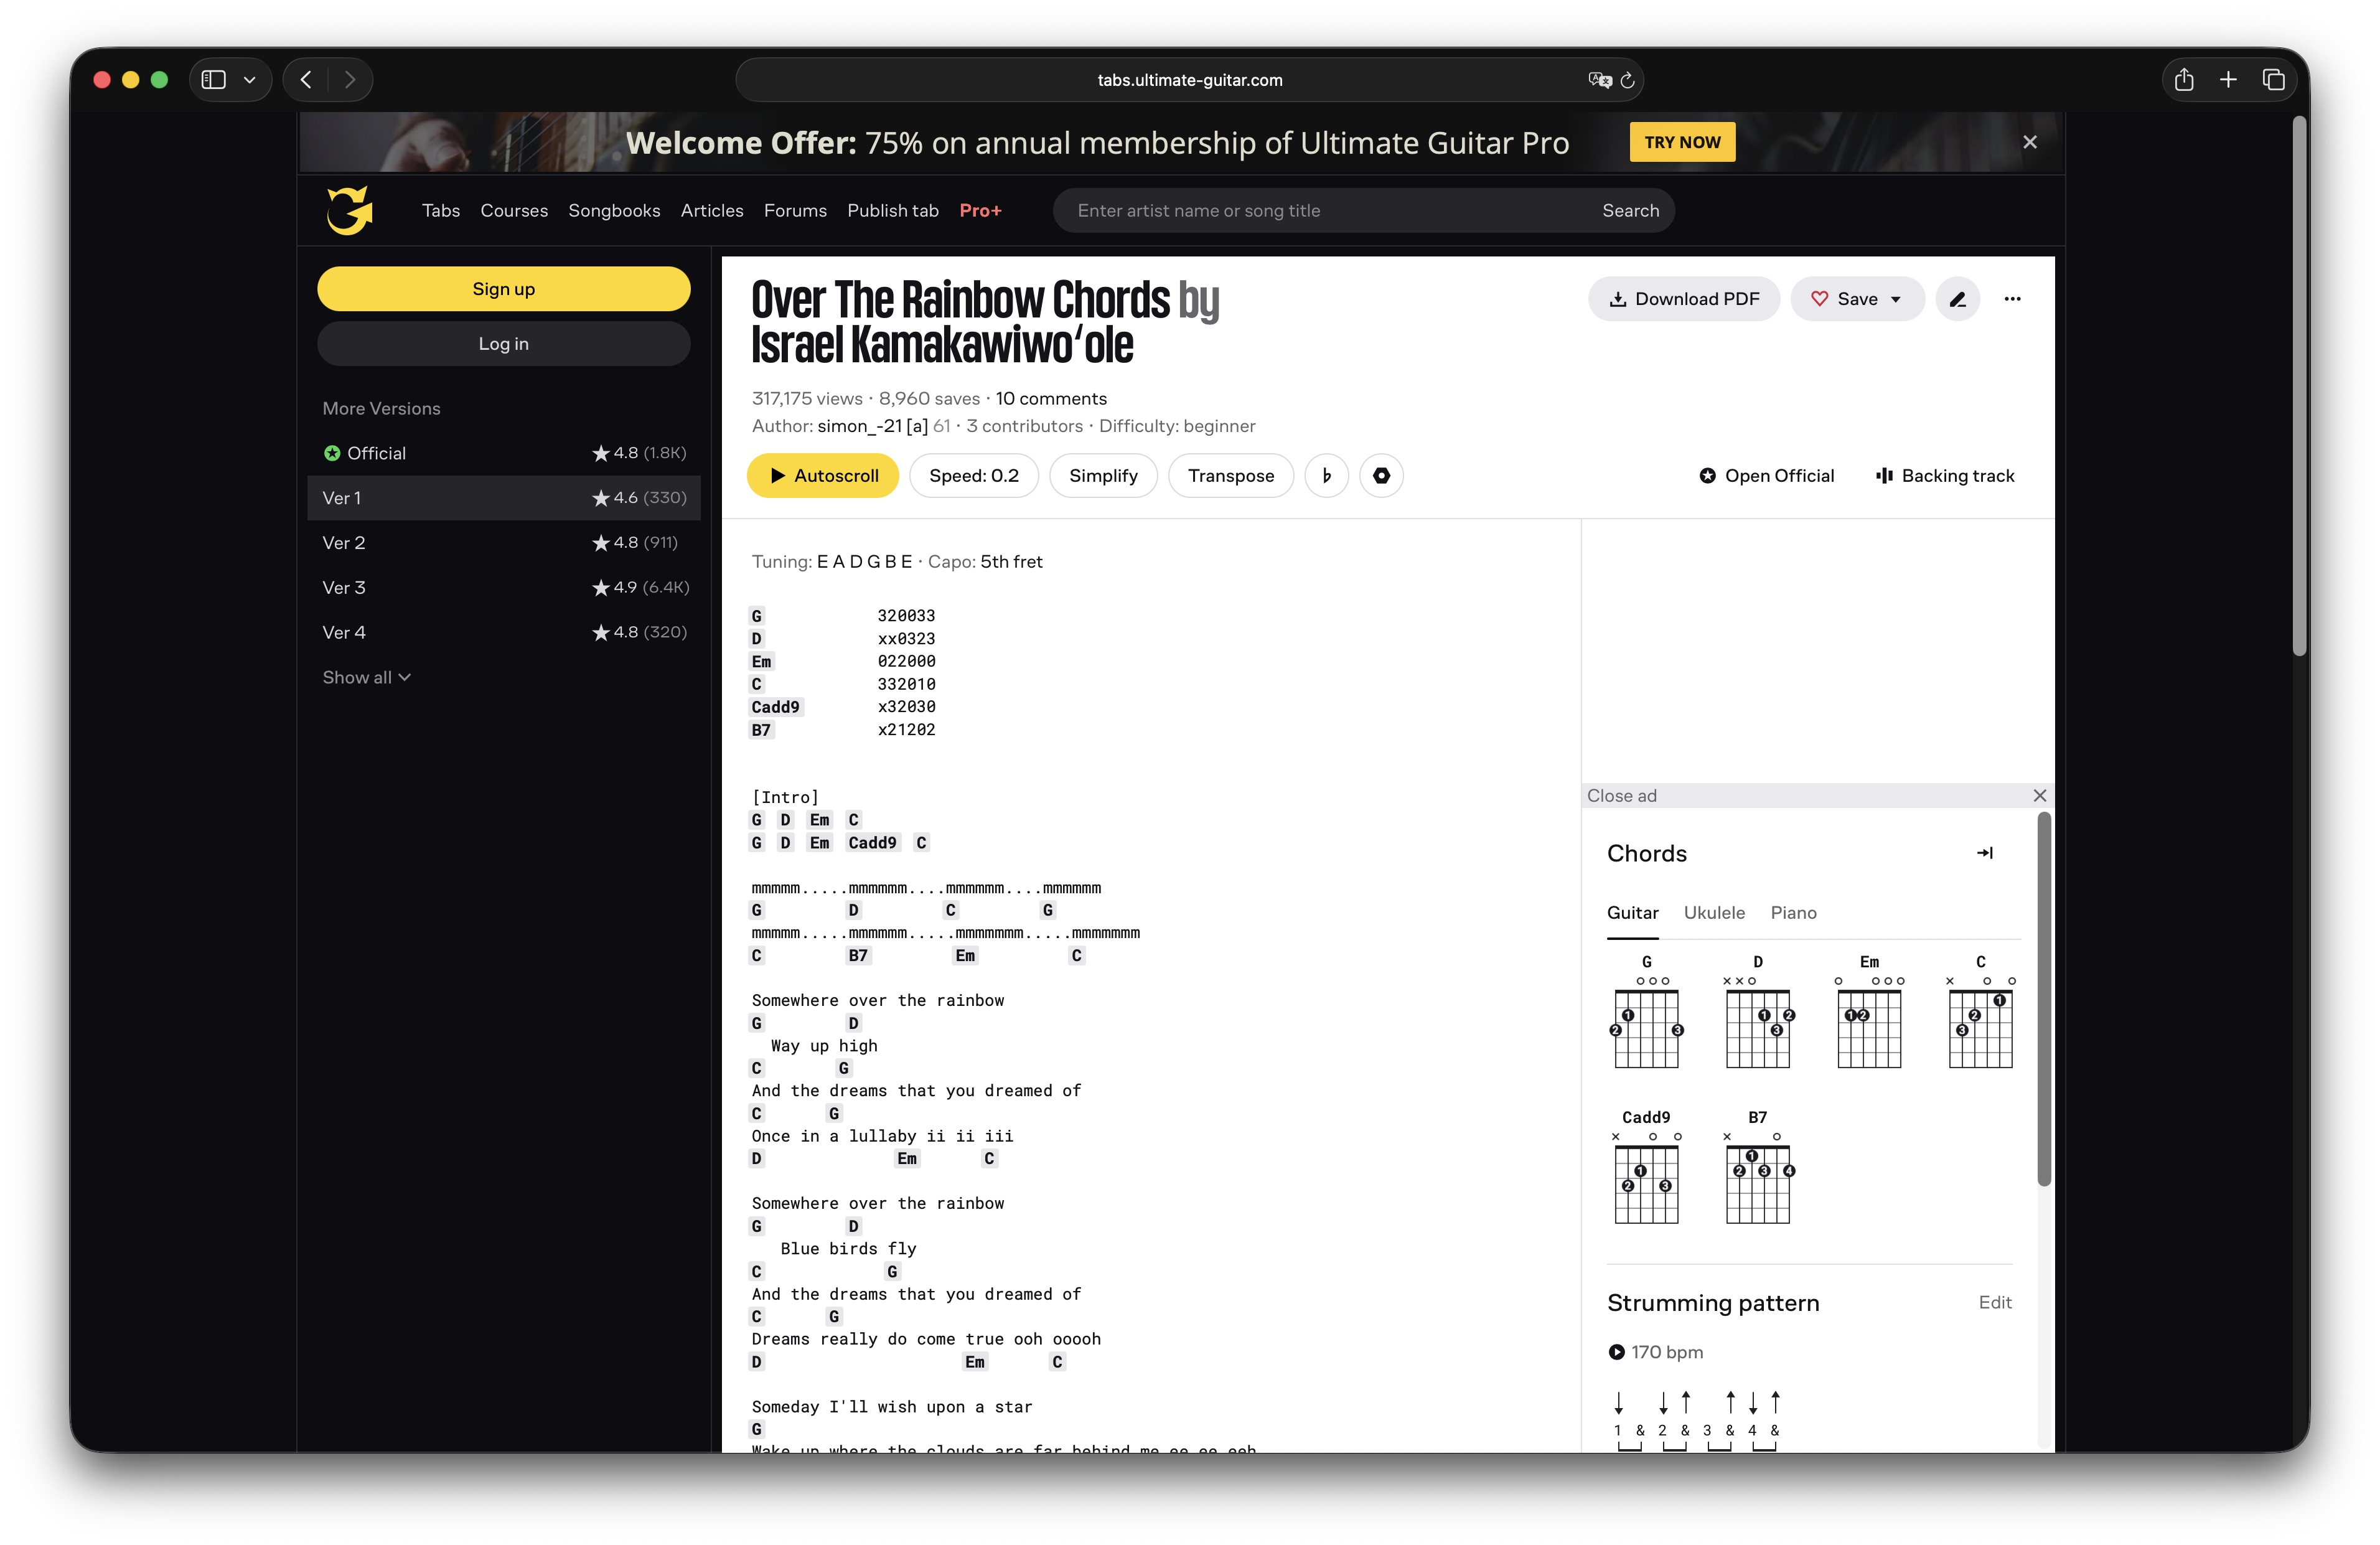
\includegraphics[width=0.8\textwidth]{Ilustraciones/estado/ultimateguitar_somewhereovertherainbow.jpeg}
        \caption{Acordes y letra de \emph{Somewhere over the rainbow}~\cite{ultimateguitar_somewhereovertherainbow} en Ultimate Guitar}
        \label{fig:ultimateguitar_somewhereovertherainbow}
    \end{subfigure}

    \caption{Páginas de Ultimate Guitar.}
    \label{fig:ultimateguitar_canciones}
\end{figure}

En conclusión, Ultimate Guitar es una aplicación web completa, ofreciendo una gran cantidad de utilidades, muchas de ellas interactivas. Su sistema de verificación a traves de la comunidad, permite además ampliar el catálogo de canciones disponibles, pudiendo encontrar varias versiones de una misma canción. No obstante, aunque gran parte de su contenido es accesible de forma gratuita, algunas funcionalidades avanzadas requieren una suscripción de pago. Para este análisis solo se tendrán en cuenta las funcionalidades que ofrezca en común con las otras alternativas seleccionadas (véase Tabla~\ref{tab:ultimateguitar_funcionalidades_usuario}).

\begin{table}[H]
    \scriptsize
    \begin{minipage}[t]{0.35\textwidth}
        \centering
        \caption{Utilidades presentes en publicaciones de Ultimate Guitar}\label{tab:ultimateguitar_utilidades_canciones}
        \begin{tabular}{l c}
            \hline
            \textbf{Utilidad} & \textbf{Existe} \\
            \hline
            Transportador & \ding{51} \\
            Lista de acordes & \ding{51} \\
            Autodesplazamiento & \ding{51} \\
            Impresión/Descarga & \ding{51} \\
            Cambio de notación &  \\
            Cambio de instrumento & \ding{51} \\
            Guardar canción & \ding{51} \\
            Guía de rasgueos & \ding{51} \\
            \hline
        \end{tabular}
    \end{minipage}
        \hfill
    \begin{minipage}[t]{0.61\textwidth}
        \centering
        \caption{Funcionalidades disponibles según el rol del usuario de Ultimate Guitar (Vis. Visitante, Reg. registrado y Sub. Suscrito)}\label{tab:ultimateguitar_funcionalidades_usuario}
        \begin{tabular}{l c c c }
            \hline
            \multirow{2}{*}{\textbf{Funcionalidad}} & \multicolumn{2}{c}{\textbf{Rol Usuario}} \\
            & Vis. & Reg. & Sub. \\
            \hline
            % --- Ejemplo de fila vacía (borra o completa) ---
            Biblioteca de canciones & \ding{51} & \ding{51} & \ding{51} \\
            Creación y edición de publicaciones &  & \ding{51} & \ding{51}  \\
            Utilidades de publicaciones & \ding{51} & \ding{51} & \ding{51} \\
            Puntuar publicaciónes &  & \ding{51} & \ding{51}  \\
            Comentar publicaciones &  & \ding{51} & \ding{51}  \\
            Solicitar nuevas canciones & & & \\
            Cursos y guías & & & \ding{51} \\
            Afinador & \ding{51} & \ding{51} & \ding{51}  \\
            Calculadora de escalas y notas &  &  &  \\
            Diccionario de acordes & & &  \\
            % ------------------------------------------------
            \hline
        \end{tabular}
    \end{minipage}
\end{table}
